\documentclass{article}

\usepackage{graphicx}
\usepackage{tikz}
\usepackage{tikzsymbols}
\usetikzlibrary{calc,patterns,shapes.geometric}
\pagestyle{empty}
\usepackage[margin=0pt]{geometry}
\geometry{papersize={14in,12in}}

\def\centerarc[#1](#2)(#3:#4:#5){\draw[#1] ($(#2)+({#5*cos(#3)},{#5*sin(#3)})$) arc (#3:#4:#5);}

\begin{document}
	\begin{figure}
		\centering
		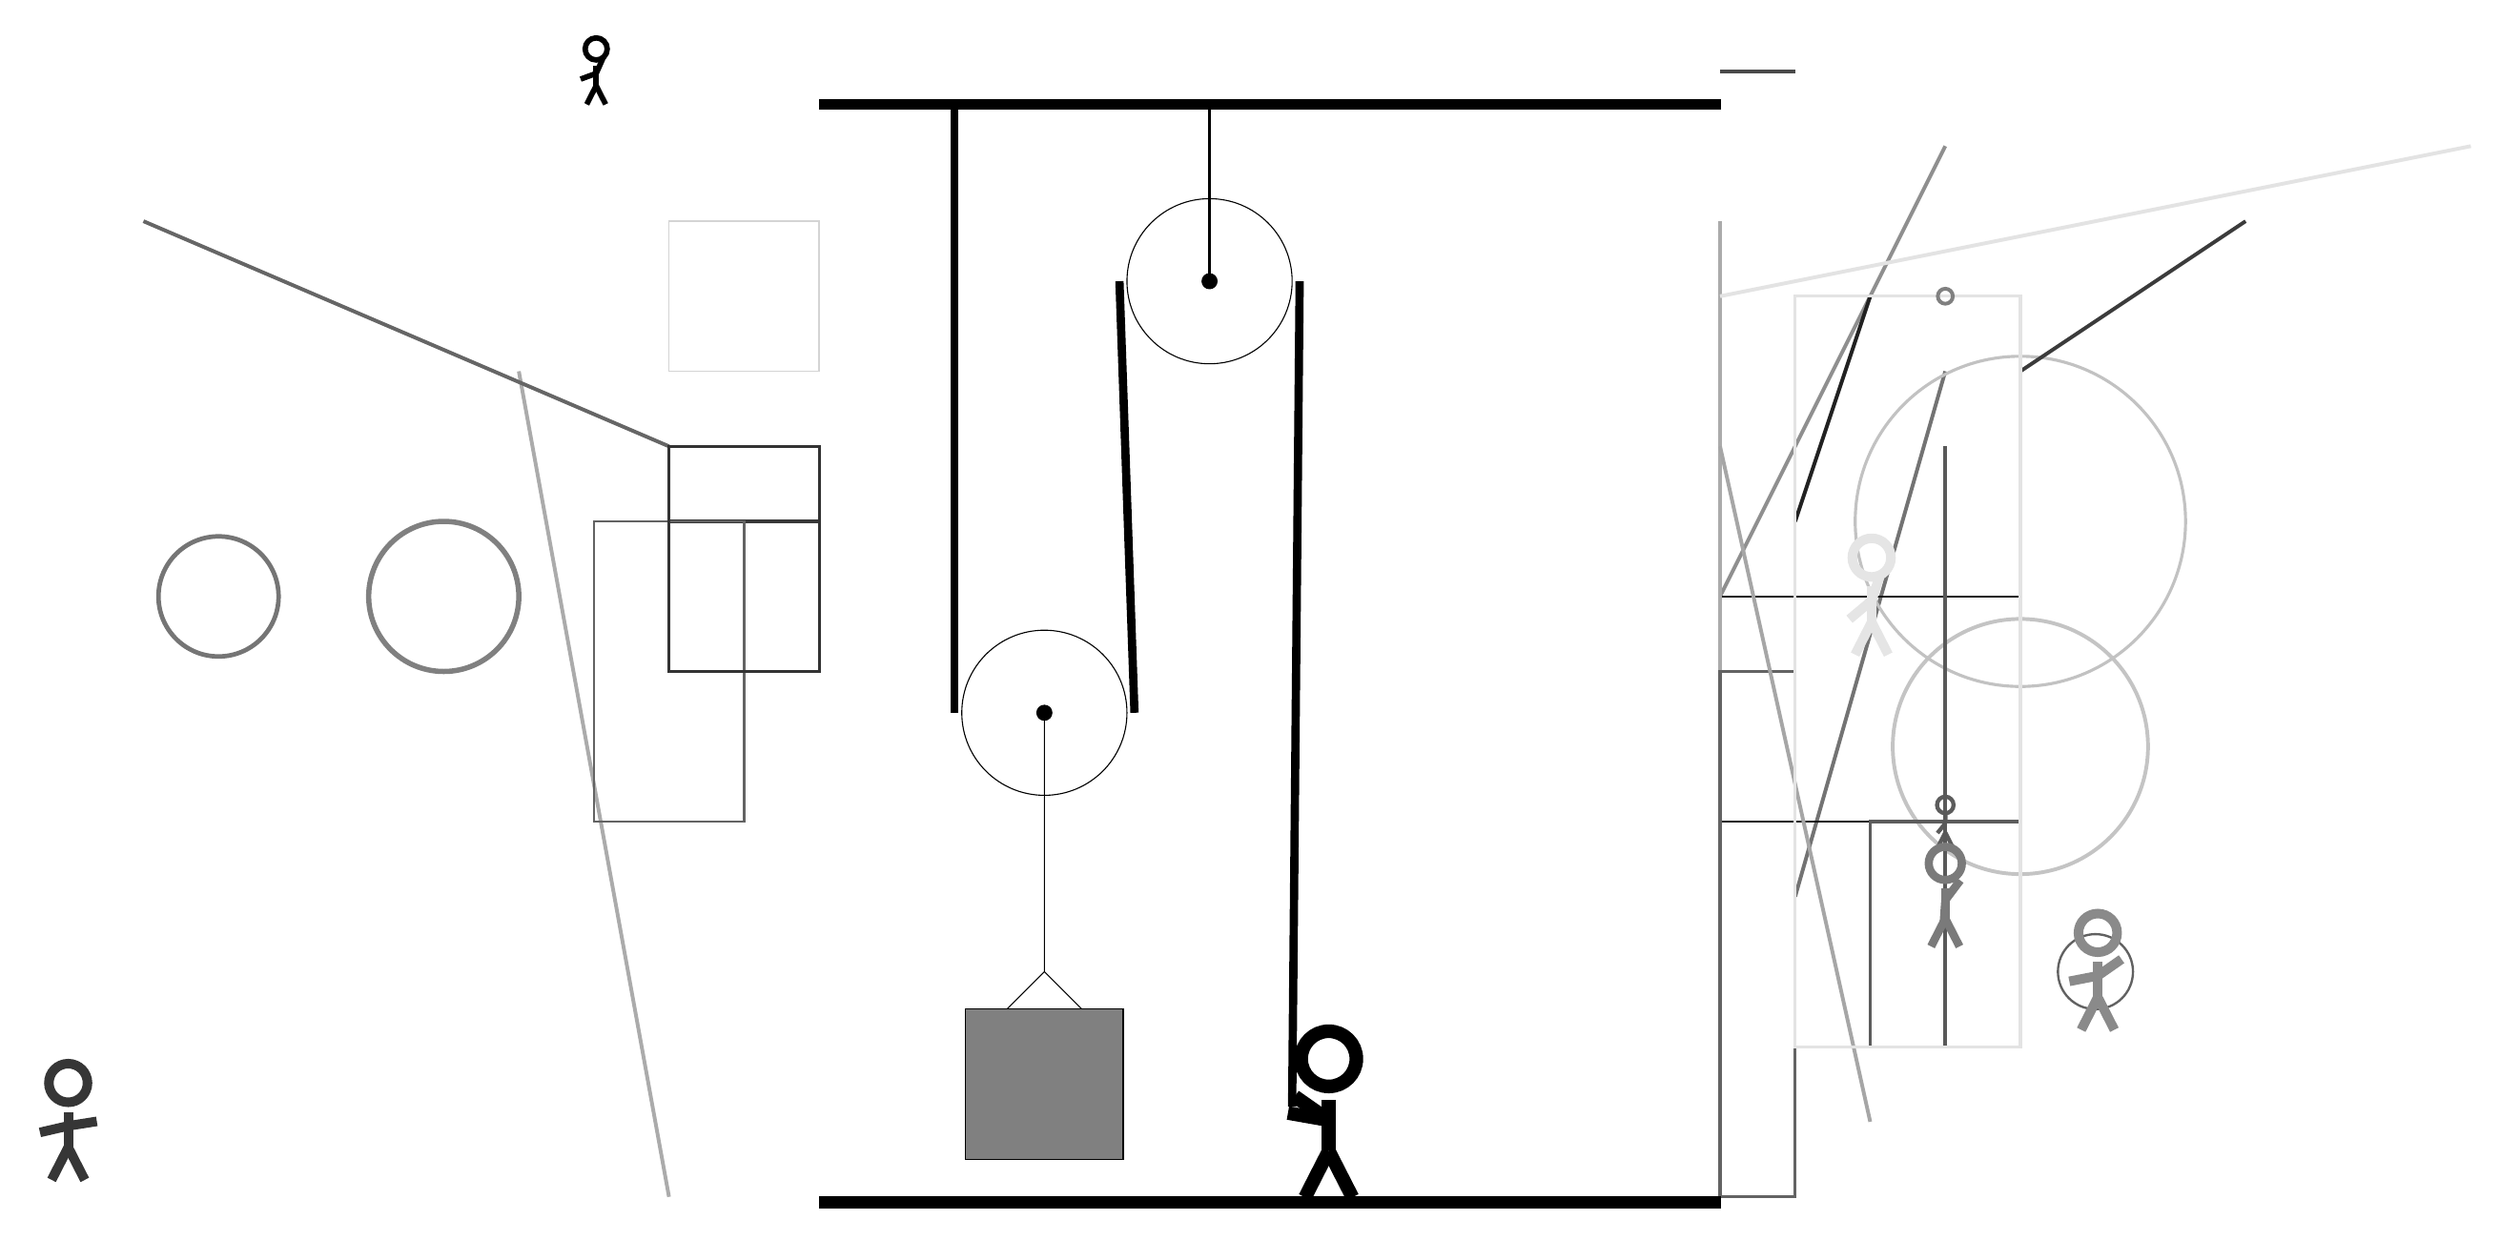
\begin{tikzpicture}
			%%%%% START %%%%%
			
			\draw[fill=black] (-2, 11.5) rectangle (10, 11.625);
			
			\draw[line width=0.5mm, color=black!33](-6, 8) -- (-4, -3);
			
			\draw[line width=0.5mm, color=black!44](13, 11) -- (10, 5);
			\draw [line width=0.5mm, color=black!23](14, 3) circle (1.7);
			\draw[line width=0.5mm, color=black!87](11, 6) -- (12, 9);
			\node[line width=0.4mm, color=black!100] at (-5, 12) {\Strichmaxerl[4][20][66]};
			\draw[line width=0.5mm, color=black!55](13, 8) -- (11, 1);
			
			\draw[line width=0.5mm, color=black!71](11, 12) -- (10, 12);
			
			\node[line width=0.4mm, color=black!64] at (13, 2) {\Strichmaxerl[3][51][88]};
			\draw[line width=0.2mm, color=black!91] (10, 2) rectangle (14, 5);
			
			\draw[line width=0.4mm, color=black!65] (10, 8) rectangle (10, 1);
			\draw[line width=0.5mm, color=black!60](-4, 7) -- (-11, 10);
			\draw[line width=0.4mm, color=black!64] (12, 2) rectangle (14, -1);
			\draw [line width=0.4mm, color=black!24](14, 6) circle (2.2);
			
			\draw [line width=0.3mm, color=black!62](15, 0) circle (0.5);
			\draw[line width=0.5mm, color=black!33](10, 10) -- (10, 2);
			\draw[line width=0.6mm, color=black!78] (-4, 6) rectangle (-2, 6);
			\draw [line width=0.6mm, color=black!54](-10, 5) circle (0.8);
			\draw[line width=0.5mm, color=black!11](10, 9) -- (20, 11);
			\draw[line width=0.4mm, color=black!61] (10, -3) rectangle (11, 4);
			\draw[line width=0.3mm, color=black!61] (-3, 2) rectangle (-5, 6);
			\draw[line width=0.5mm, color=black!35](10, 7) -- (12, -2);
			
			\draw [line width=0.7mm, color=black!50](-7, 5) circle (1.0);
			\node[line width=0.7mm, color=black!46] at (15, 0) {\Strichmaxerl[7][11][35]};
			\draw[line width=0.4mm, color=black!80] (-2, 7) rectangle (-4, 4);
			\draw[line width=0.5mm, color=black!65](13, 7) -- (13, -1);
			\draw[line width=0.5mm, color=black!77](14, 8) -- (17, 10);
			\node[line width=0.6mm, color=black!52] at (13, 1) {\Strichmaxerl[6][86][53]};
			\draw[line width=0.4mm, color=black!11] (11, -1) rectangle (14, 9);
			\draw [line width=0.5mm, color=black!50](13, 9) circle (0.1);
			
			\draw[line width=0.2mm, color=black!17] (-2, 8) rectangle (-4, 10);
			\node[line width=0.7mm, color=black!10] at (12, 5) {\Strichmaxerl[7][40][72]};
			\node[line width=0.2mm, color=black!79] at (-12, -2) {\Strichmaxerl[7][13][9]};
			
			\draw (3.2, 9.2) circle (1.1);
			\draw[fill=black] (3.2, 9.2) circle (0.1);
			\draw[thick] (3.2, 9.2) -- (3.2, 11.5);
			
			\draw (1, 3.45) circle (1.1);
			\draw[fill=black] (1, 3.45) circle (0.1);
			
			\draw (1, 3.45) -- (1, 0.0) -- (0.5, -0.5);
			\draw (1, 0.0) -- (1.5, -0.5);
			\draw[fill=black!50] (-0.05, -0.5) rectangle (2.05, -2.5);
			
			\draw[line width=1.1mm] (-0.2, 11.5) -- (-0.2, 3.45);
			\centerarc[line width=1.1mm](1, 3.45)(180:360:1.2000000000000002);
			\draw[line width=1.1mm](2.2, 3.45) -- (2.0, 9.2);
			\centerarc[line width=1.1mm](3.2, 9.2)(0:180:1.2000000000000002);
			\draw[line width=1.1mm](4.4, 9.2) -- (4.3, -1.8);
			
			\node at (4.7, -1.9) {\Strichmaxerl[10][-35][170]};
			
			\draw[fill=black] (-2, -3) rectangle (10, -3.15);
			
			%%%%% END %%%%%
		\end{tikzpicture}
	\end{figure}	
\end{document}